\section{Wrap-up}
\begin{frame}{DDPG Follow-up}
\begin{itemize}
    \footnotesize
    \item Model the actor as the $\arg\max$ of a convex function
    \begin{itemize}
        \item \emph{Continuous Deep Q-Learning with Model-based Acceleration} (Shixiang Gu, Timothy Lillicrap, Ilya Sutskever, Sergey Levine, ICML 2016)
        \item \emph{Input Convex Neural Networks} (Brandon Amos, Lei Xu, J.~Zico Kolter, ICML 2017)
    \end{itemize}
    \item Q-value overestimation
    \begin{itemize}
        \item \emph{Addressing Function Approximation Error in Actor-Critic Methods (TD3)} (Scott Fujimoto, Herke van Hoof, David Meger, ICML 2018)
    \end{itemize}
    \item Stochastic policy search
    \begin{itemize}
        \item \emph{Soft Actor-Critic: Off-Policy Maximum Entropy Deep Reinforcement Learning with a Stochastic Actor} (Tuomas Haarnoja, Aurick Zhou, Pieter Abbeel, Sergey Levine, ICML 2018)
    \end{itemize}
\end{itemize}
\vspace{0.2em}
\begin{columns}[T]
\begin{column}{0.5\textwidth}
\begin{figure}
    \centering
    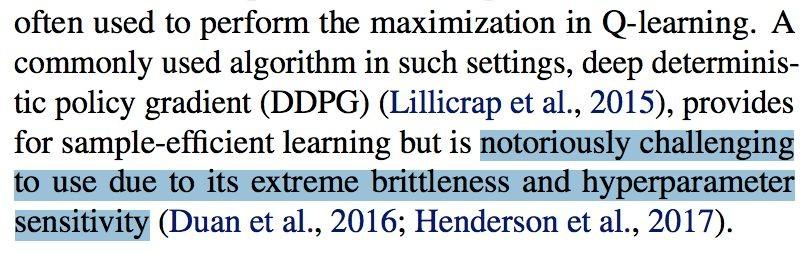
\includegraphics[width=\linewidth,height=0.22\textheight,keepaspectratio]{images/ddpg/figures/followup-quote-1.jpg}
\end{figure}
\end{column}
\begin{column}{0.5\textwidth}
\begin{figure}
    \centering
    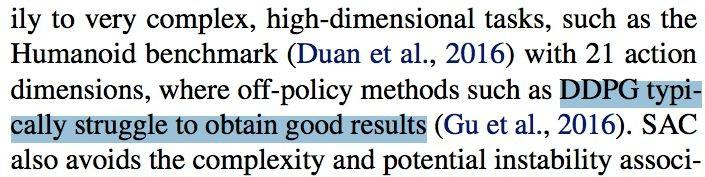
\includegraphics[width=\linewidth,height=0.22\textheight,keepaspectratio]{images/ddpg/figures/followup-quote-2.jpg}
\end{figure}
\end{column}
\end{columns}
\end{frame}
